\ylDisplay{Õõnes kera} % Ülesande nimi
{Tanel Kiis} % Autor
{piirkonnavoor} % Voor
{2013} % Aasta
{G 9} % Ülesande nr.
{8} % Raskustase
{
% Teema: Dünaamika
\ifStatement
Jukul on rauast kera
($\varrho_\mathrm{Fe}=\SI{7,9}{\gram\per\centi\meter\cubed}$) raadiusega
$r=\SI{10}{\centi\meter}$ ja massiga $m=\SI{30}{\kilo\gram}$. Juku teab, et kera
sees on sfääriline õõnsus, mille keskpunkti kaugust $d$ kera keskpunktist ta üritab
leida. Selleks riputas ta kuuli kaks korda nööri otsa rippuma, kasutades
riputuskohtadeks kera vastaspunkte. Ühel korral moodustas neid kinnituspunkte
ühendav telg horisondiga nurga $\alpha=\SI{60}{\degree}$, teisel korral aga nurga
$\beta=\SI{45}{\degree}$. Leidke $d$.
\fi


\ifHint
Õõnsusega kera saab vaadelda positiivse tihedusega täidetud kera ja õõnsuse suuruse negatiivse tihedusega kera superpositsioonina. Sellisel juhul saab mugavalt kirja panna jõumomentide tasakaalu mõlema stsenaariumi jaoks.
\fi


\ifSolution
\begin{center}
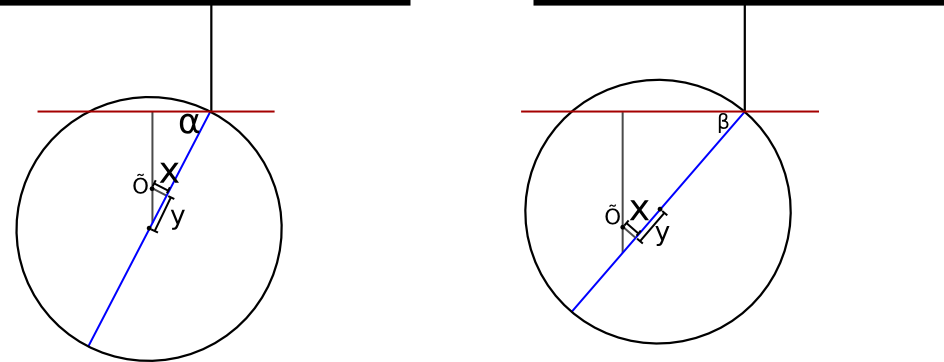
\includegraphics[width=\textwidth]{2013-v2g-09-kera.png}
\end{center}

Kui tegemist poleks õõnsa keraga, oleks selle mass $M=\frac{4}{3}\pi r^3 = \SI{33}{kg}$. Mudeldame õõnsusega kera kui tervet kera, mille sees on negatiivse massiga $m'=\SI{3}{kg}$ kera. Kera pöörab ennast nii, et tema masskese jääks kinnituspunkti alla. Olge õõnsuse keskpunkti (Õ) asukoha koordinaadid kera keskpunkti suhtes $x$ ja $y$. Nende leidmiseks kasutame jõumomentide tasakaalu nööri kinnituspunkti suhtes. Saame võrrandisüsteemi:
\[Mr \cos \alpha = m'(r-y+x \tan \alpha) \cos \alpha,\]
\[Mr \cos \beta = m'(r+y+x \tan \beta) \cos \beta.\]
Õõnsuse ja kera keskpunktide vaheline kaugus on $d=\sqrt{x^2+y^2}$,
\[ d=\frac{2r(\frac{M}{m'}-1)}{\tan\alpha+\tan\beta}\sqrt{1+\frac{1}{4}(\tan\alpha-\tan\beta)^2} = \SI{0,8}{cm}. \]
\fi


\ifEngStatement
% Problem name: Hollow ball
Juku has an iron ball ($\varrho_\mathrm{Fe}=\SI{7,9}{\gram\per\centi\meter\cubed}$) of radius $r=\SI{10}{\centi\meter}$ and mass $m=\SI{30}{\kilo\gram}$. Juku knows that inside the ball there is a spherical hollowness and he wants to find the distance $d$ from the center of the ball to the center of the hollowness. To do that he hanged the ball to a thread two times, using two opposite points on the ball as the hanging points. At the first time, the axis that connected the two hanging points formed an angle $\alpha=\SI{60}{\degree}$ with respect to the horizontal axis, the second time that angle was $\beta=\SI{45}{\degree}$. Find $d$.
\fi


\ifEngHint
The hollowed sphere can be looked at as a superposition of a filled sphere with positive density and a sphere with the size of the cavity that has negative density. In this case the torque balance can be easily written down for both scenarios.
\fi


\ifEngSolution
\begin{center}
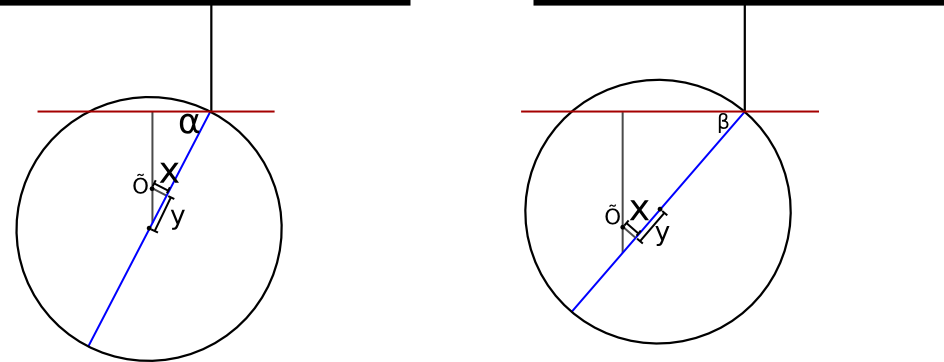
\includegraphics[width=\textwidth]{2013-v2g-09-kera}
\end{center}
If we would not be dealing with a hollow ball then its mass would be $M=\frac{4}{3}\pi r^3 = \SI{33}{kg}$. We will model the hollow ball as a whole ball that has a ball with a negative mass $m'=\SI{3}{kg}$ inside. The ball rotates itself so that its center of mass stays below the attachment point. Let the coordinates of the hollow’s center (Õ) with respect to the ball’s center be $x$ and $y$. To find these we will use torque balance with respect to the thread’s attachment point. We will get system of equations:
\[Mr \cos \alpha = m'(r-y+x \tan \alpha) \cos \alpha,\] 
\[Mr \cos \beta = m'(r+y+x \tan \beta) \cos \beta.\]
The distance between the centers of the hollow and the ball is $d=\sqrt{x^2+y^2}$.
\[ d=\frac{2r(\frac{M}{m'}-1)}{\tan\alpha+\tan\beta}\sqrt{1+\frac{1}{4}(\tan\alpha-\tan\beta)^2} = \SI{0,8}{cm}. \]
\fi
}